\documentclass[11pt,a4paper]{article}

\usepackage[T1]{fontenc}
\usepackage[utf8]{inputenc}
\usepackage{lmodern}
\usepackage{microtype}
\usepackage{amsmath,amssymb,amsthm}
\usepackage{booktabs}
\usepackage{multirow}
\usepackage{array}
\usepackage{graphicx}
\usepackage{hyperref}
\usepackage{xcolor}
\usepackage{enumitem}
\usepackage{geometry}
\usepackage{algorithm}
\usepackage{algpseudocode}
\usepackage{listings}
\usepackage{tikz}
\usetikzlibrary{positioning,arrows.meta,fit,shapes.geometric}

\geometry{margin=2.4cm}

\hypersetup{
  colorlinks=true,
  linkcolor=blue!55!black,
  citecolor=blue!55!black,
  urlcolor=blue!55!black
}

\lstset{
  basicstyle=\ttfamily\footnotesize,
  breaklines=true,
  frame=single,
  framerule=0.4pt,
  rulecolor=\color{gray!40},
  showstringspaces=false,
  columns=fullflexible,
  keepspaces=true,
}

\newcommand{\REX}{\textsc{Rex1}\xspace}
\providecommand{\xspace}{}

\title{\textbf{REX1: A Parameter-Efficient Recurrent Looped Language Model}\\[0.5em]
\large Architecture, Multi-Stage Training Pipeline, and Specialist Release}
\author{REX Research Team}
\date{May 2026}

\begin{document}
\maketitle

\begin{abstract}
We present \textbf{REX1}, a 269M-parameter recurrent looped decoder-only language model
designed for parameter-efficient reasoning, edge deployment, and downstream
specialization into chat, code, mathematics, and vision–language–action (VLA)
backbones. REX1 reuses a single 8-layer transformer stack for $R{=}4$ latent
recurrence steps and is trained with an Ouro-style entropy-regularized depth
allocation objective, in which a learned per-step exit gate produces a
distribution over recurrence depths that weights per-step cross-entropy losses.

Training follows a five-stage \emph{Ouro pipeline} adapted to research-scale
compute (2$\times$ NVIDIA RTX Pro 6000): (i) broad pretraining on
$\sim$2.25B SmolLM2 tokens, (ii) continual-training (CT) annealing on a
high-quality DCLM-Edu/Nemotron-Math/MegaMath/OpenCoder mixture with reduced
learning rate and exit-gate entropy coefficient, (iii) mid-training on a curated
code/math/CoT mix with 20\% pretraining replay, (iv) four parallel specialist
supervised fine-tuning (SFT) branches initialized from the same mid-training
checkpoint, and (v) a planned reinforcement-learning stage using sparse
verifiable rewards (for math/code) and direct preference optimization (for
chat).

At pretraining step 40{,}000 ($\approx$5.2B tokens processed), REX1 already
reaches HellaSwag~35.5\% and ARC-Easy~43.5\% under a continuation-loss
multiple-choice protocol. Stage~2 continues from this checkpoint with a
dedicated high-quality annealing corpus built from DCLM-Edu,
Nemotron-CC-Math, MegaMath-Web-Pro, and OpenCoder data.
While these absolute numbers remain below fully-trained Pythia-410M
(58$\times$ more pretraining tokens) and SmolLM2-360M (hundreds of times more
tokens), the trajectory indicates that the LoopLM family scales reasonably at
small parameter budgets when paired with a careful curriculum.

We release the full training code, all YAML stage configurations, data
download recipes, evaluation harness, and this report to support
reproducibility and downstream adaptation. The accompanying repository covers
the pipeline end-to-end, including a text-only SFT recipe (\textsc{Rex1-VLA-Backbone})
that steers the base model toward embodied robotics language without requiring
visual data at this stage.
\end{abstract}

\tableofcontents
\newpage

%==============================================================================
\section{Introduction}
%==============================================================================

\subsection{Motivation}

Modern large language models (LLMs) achieve their capabilities largely through
increases in parameter count and training-token budgets. A 7B-parameter dense
transformer trained on several trillion tokens dominates the open-source
landscape, but such models are difficult to deploy on edge devices, fine-tune
for specialized downstream tasks (robotics, on-device assistants), or to
iterate on as research artifacts.

\emph{Looped} (or recurrent) language models~\cite{ouro2025,deth} offer one
appealing direction at small scale: a single transformer block stack is
applied $R$ times to refine the latent representation before token prediction.
Effective \emph{depth} is decoupled from parameter \emph{count}: instead of
stacking $L$ layers with independent weights, one stacks $N_l$ blocks and
recurses $R$ times for an effective depth of $R \cdot N_l$. The cost is paid
at inference (more compute per token) rather than in memory (more weights to
store, load, or quantize), which is precisely the tradeoff one wants on a
phone or microcontroller.

The Ouro family~\cite{ouro2025} extends this idea with a learned \emph{depth
allocation} objective: an exit gate at every recurrence step produces a
distribution over termination depths, allowing easy tokens to terminate
early and hard tokens to use more compute. The training objective combines
per-step cross-entropy loss weighted by the exit distribution with a
KL-regularization term toward a uniform prior over depths, preventing
collapse into a single-step model.

\subsection{Goals of REX1}

\REX is intended as a small, fully open, multi-stage LoopLM with three explicit
research goals:

\begin{enumerate}[leftmargin=*]
  \item \textbf{Parameter-efficient reasoning at small scale.}
    Demonstrate that a 269M-parameter looped model, trained on a research-scale
    token budget ($\sim$10B tokens across all stages), can produce
    competitive results on standard multiple-choice reasoning benchmarks.

  \item \textbf{Edge-friendly deployment.}
    Provide a model family that fits within the memory and latency budgets of
    consumer hardware, exploiting (a) grouped-query attention, (b) inference-time
    early exit, and (c) compatibility with standard quantization (Q4\_K\_M, AWQ).

  \item \textbf{Multi-specialist release from a shared base.}
    Use a mid-training checkpoint as a launching point for four parallel
    specialists---\textsc{Rex1-Chat}, \textsc{Rex1-Code}, \textsc{Rex1-Math},
    and \textsc{Rex1-VLA-Backbone}---each branched from the same checkpoint
    rather than sequentially stacked.
\end{enumerate}

\subsection{Contributions}

This report makes the following technical contributions:

\begin{enumerate}[leftmargin=*]
  \item A complete, self-contained PyTorch implementation of a small-scale
    Ouro-style LoopLM, including: (i) shared-weight recurrence with optional
    early-exit at inference, (ii) per-step LM-head readouts and exit-gate
    KL regularization, (iii) grouped-query attention with rotary
    positional embeddings, and (iv) sandwich normalization.
  \item A reproducible five-stage training pipeline, including YAML
    configurations for pretraining, CT annealing, mid-training, and four
    parallel SFT branches.
  \item A token-stream data engineering tool that handles flat text columns,
    Jinja-style templates, multi-turn conversation columns, and an
    \emph{inter-stage replay} mode that samples token chunks from previous
    stages' packed bins to mitigate forgetting during mid-training and SFT.
  \item A lightweight evaluation harness implementing continuation-loss
    multiple-choice scoring on HellaSwag, ARC, SciQ, OpenBookQA,
    WinoGrande, PIQA, and BoolQ, with inline-during-training and
    standalone modes.
  \item A documented \emph{text-only} SFT recipe designed to steer the base
    model toward embodied robotics language as a backbone for later
    vision-language-action specialization.
  \item Preliminary results characterizing the model after stage~1 pretraining
    at $\sim$5.2B tokens, with explicit comparison
    caveats regarding our continuation-loss MC evaluation versus the
    log-likelihood scoring used in standard harnesses.
\end{enumerate}

\subsection{Scope and Non-Goals}

This is an engineering and reproducibility report rather than an empirical
study of looped LMs at scale. We do not claim parity with frontier models, nor
do we present ablations decomposing the contributions of architectural
choices. The data mixtures, hyperparameters, and pipeline are deliberately
simple and conservative, prioritizing transparency and ease of further
modification.

%==============================================================================
\section{Related Work}
%==============================================================================

\subsection{Looped and Recurrent Transformers}

The idea of reusing transformer block weights across multiple passes appears
in Universal Transformers~\cite{universal-transformer}, Albert~\cite{albert}
(layer sharing for parameter efficiency), and the recent Ouro
family~\cite{ouro2025}. Block-recurrent
transformers~\cite{block-recurrent-transformer} share a related motivation
but apply recurrence over chunks of the sequence rather than refining the
latent representation in place. Latent reasoning models such as
Coconut~\cite{coconut} and Quiet-STaR~\cite{quietstar} also iterate on hidden
state but typically introduce special ``thought'' tokens rather than weight
sharing per se.

Two ingredients distinguish the Ouro recipe and \REX:
(i) \emph{step-level supervision} via per-step LM-head losses, which avoids
the credit-assignment difficulty of supervising only the final readout, and
(ii) a \emph{learned exit-gate distribution} regularized toward uniformity,
which provides a principled mechanism for adaptive compute without
introducing brittle thresholding heuristics during training.

\subsection{Multi-Stage Pretraining and Mid-Training}

The two- or three-stage pretraining recipe (broad data $\rightarrow$
annealing on cleaner data $\rightarrow$ post-training) has become standard
practice~\cite{nemotron,olmo2,llama3}. Mid-training---an intermediate
phase between annealing and instruction tuning that uses curated
math/code/reasoning data with optional general-data replay---has been
explicitly described in OLMo~2~\cite{olmo2}, Yi~\cite{yi}, and the recent
surveys~\cite{midtrain2025,midtrain-survey-23081}, and rigorously analyzed
in Springer et al.~\cite{springer-midtrain}. \REX follows this convention
explicitly with named stages and replay support.

\subsection{Parallel Specialist Models from a Shared Base}

Branching multiple specialists from a single high-quality base checkpoint is
the pattern used by Code Llama~\cite{codellama}, which forks from a Llama 2
base rather than stacking on top of the chat model. The same pattern is used
in many instruction-tuned releases (general chat, code, math) which all
initialize from a shared base or mid-training checkpoint. We follow this
design rather than sequential stacking to avoid the forgetting/interference
issues induced by long SFT runs on narrow data distributions.

\subsection{Vision–Language–Action Backbones}

Modern VLA systems (RT-2~\cite{rt2}, OpenVLA~\cite{openvla}) attach a vision
encoder and an action head to a language model backbone. The language
model is usually a general instruct model, which is not ideal because it has
been trained for chat-style dialog rather than for embodied imperative
language, spatial reasoning, and action sequences. We provide a text-only
SFT recipe (\textsc{Rex1-VLA-Backbone}) that steers the LM toward
robotics-friendly behavior \emph{before} any visual data is introduced,
following the spirit of language-conditioned policy pretraining in
RT-1~\cite{rt1} and Octo~\cite{octo}.

%==============================================================================
\section{Model Architecture}
%==============================================================================

\subsection{Notation}

We use lowercase italics for scalars, lowercase bold for vectors, and
uppercase bold for matrices. Let $B$ denote batch size, $T$ sequence length,
$d \equiv d_{\mathrm{model}}$ the model dimension, $V$ the vocabulary size,
$H$ the number of attention heads, $H_k$ the number of KV heads in
grouped-query attention, and $d_h = d / H$ the per-head dimension. Let
$N_l$ denote the number of transformer blocks and $R$ the number of
recurrence steps.

\subsection{Overview}

\REX is a decoder-only causal language model. Unlike a standard $L$-layer
transformer that applies $L$ distinct blocks sequentially, \REX applies the
\emph{same} stack of $N_l = 8$ blocks $R = 4$ times in a recurrence loop,
producing a list of hidden states $\bigl(\mathbf{h}^{(1)}, \ldots,
\mathbf{h}^{(R)}\bigr)$. The effective network depth is therefore
$R \cdot N_l = 32$ block applications, with the parameter cost of an 8-layer
model.

Step identity is supplied via a learned step embedding $\mathbf{s}_r \in
\mathbb{R}^{d}$ added to the latent representation at the start of recurrence
step $r$. An exit-gate head produces a probability distribution over depths
that is used both for training-time loss weighting and for inference-time
early termination.

A schematic of one forward pass is shown in Figure~\ref{fig:arch}.

\begin{figure}[h]
\centering
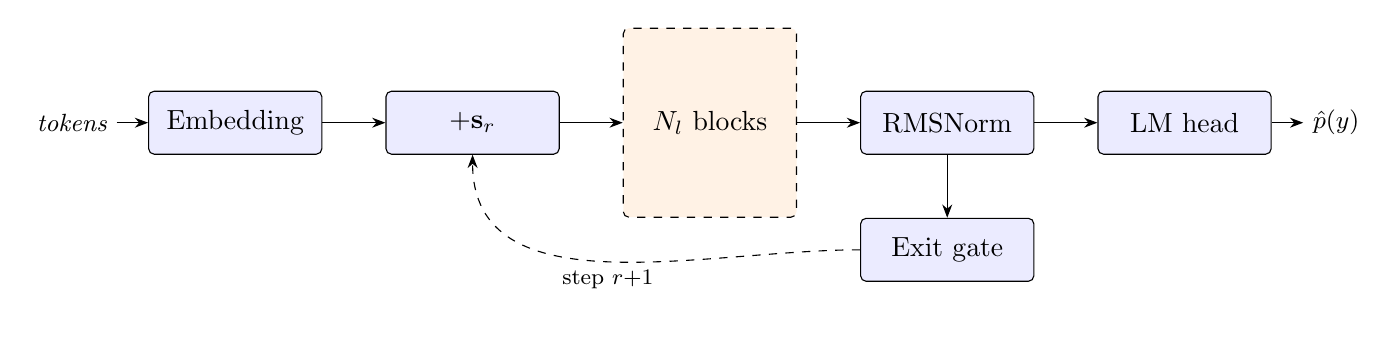
\begin{tikzpicture}[
  >=Stealth,
  node distance=8mm,
  block/.style={draw, rounded corners=2pt, minimum width=22mm, minimum height=8mm, fill=blue!8},
  loop/.style={draw, rounded corners=2pt, minimum width=22mm, minimum height=24mm, fill=orange!10, dashed},
  io/.style={draw=none, font=\small\itshape},
]
\node[io] (tok) {tokens};
\node[block, right=4mm of tok] (emb) {Embedding};
\node[block, right=of emb] (step) {$+\mathbf{s}_r$};
\node[loop, right=of step] (blocks) {$N_l$ blocks};
\node[block, right=of blocks] (norm) {RMSNorm};
\node[block, right=of norm] (head) {LM head};
\node[block, below=of norm] (gate) {Exit gate};
\node[io, right=4mm of head] (out) {$\hat p(y)$};
\draw[->] (tok) -- (emb);
\draw[->] (emb) -- (step);
\draw[->] (step) -- (blocks);
\draw[->] (blocks) -- (norm);
\draw[->] (norm) -- (head);
\draw[->] (head) -- (out);
\draw[->] (norm) -- (gate);
\draw[->, dashed] (gate.west) to[out=180, in=-90] node[below, font=\footnotesize] {step $r$$+$1} (step.south);
\end{tikzpicture}
\caption{One forward pass of \REX. The $N_l$ shared blocks (orange box) are
applied $R$ times. At each step, the post-normalization hidden state feeds
both the LM head (for training-time per-step loss) and the exit gate (for
depth allocation).}
\label{fig:arch}
\end{figure}

\subsection{Tokenizer}

\REX uses the SmolLM2-360M~\cite{smollm2} tokenizer, a 49{,}152-piece byte-pair
encoding (BPE) trained on a mixture of English web and code. This choice
provides:
(i) competitive compression on natural language and code,
(ii) availability of a well-documented chat template system, and
(iii) a stable HuggingFace tokenizer artifact that is easy to redistribute.

\subsection{Embeddings}

Token embeddings $\mathbf{E} \in \mathbb{R}^{V \times d}$ are tied with the
LM-head projection. Tied embeddings save $V \cdot d \approx 75.5\mathrm{M}$
parameters and are standard in models in this size range.

\subsection{Self-Attention}

\paragraph{Grouped-query attention.}
Following \cite{gqa}, \REX uses $H = 16$ query heads and $H_k = 4$ KV heads,
with each KV head shared across $H/H_k = 4$ query heads via repeat. Queries
and keys are projected to $H \cdot d_h$ and $H_k \cdot d_h$ respectively
(with $d_h = 96$ when $d = 1536$); values share the same dimension as keys.

For a sequence $\mathbf{X} \in \mathbb{R}^{T \times d}$, the projections are
\begin{equation}
\mathbf{Q} = \mathbf{X}\mathbf{W}_Q, \quad
\mathbf{K} = \mathbf{X}\mathbf{W}_K, \quad
\mathbf{V} = \mathbf{X}\mathbf{W}_V,
\end{equation}
with $\mathbf{W}_Q \in \mathbb{R}^{d \times H d_h}$ and
$\mathbf{W}_K, \mathbf{W}_V \in \mathbb{R}^{d \times H_k d_h}$, all without
bias.

\paragraph{Rotary positional embeddings.}
Following \cite{rope}, we apply rotary embeddings to $\mathbf{Q}$ and
$\mathbf{K}$ before the dot product. For each pair of head dimensions
$(2i, 2i+1)$ and position $p$, the rotation matrix is
\begin{equation}
\mathbf{R}_{p,i} = \begin{pmatrix} \cos(p\, \omega_i) & -\sin(p\, \omega_i) \\
\sin(p\, \omega_i) & \cos(p\, \omega_i) \end{pmatrix},
\quad
\omega_i = \theta^{-2i / d_h},
\end{equation}
with base $\theta = 50{,}000$. We use the standard ``rotate-half'' implementation
that interleaves even and odd dimensions.

\paragraph{Causal attention.}
Standard scaled-dot-product attention is computed via
PyTorch's \texttt{scaled\_dot\_product\_attention} with the causal mask flag,
which routes to a fused kernel (FlashAttention-style) when available.

\paragraph{Optional block-local attention.}
The implementation supports a non-overlapping block-local causal mask
(\texttt{local\_block\_size > 0}) to allow ablations with limited
receptive field. The default is global causal attention (\texttt{local\_block\_size = 0}).

\subsection{SwiGLU Feed-Forward}

Each block contains a SwiGLU~\cite{swiglu} feed-forward network:
\begin{equation}
\mathrm{FFN}(\mathbf{x}) = \mathbf{W}_2 \bigl( \mathrm{SiLU}(\mathbf{W}_1 \mathbf{x}) \odot \mathbf{W}_3 \mathbf{x} \bigr),
\end{equation}
with $\mathbf{W}_1, \mathbf{W}_3 \in \mathbb{R}^{d \times d_{\mathrm{ffn}}}$
and $\mathbf{W}_2 \in \mathbb{R}^{d_{\mathrm{ffn}} \times d}$. We set
$d_{\mathrm{ffn}} = 3968 \approx 2.58\,d$, slightly below the
$\frac{8}{3}d$ heuristic, chosen to round to a multiple of 64.

\subsection{Normalization}

We use RMSNorm~\cite{rmsnorm}:
\begin{equation}
\mathrm{RMSNorm}(\mathbf{x}) = \frac{\mathbf{x}}{\sqrt{\frac{1}{d}\sum_i x_i^2 + \epsilon}} \odot \boldsymbol{\gamma},
\end{equation}
with learnable scale $\boldsymbol{\gamma} \in \mathbb{R}^d$ and
$\epsilon = 10^{-5}$. The computation is performed in float32 and cast back
to the input dtype to preserve numerical stability under bf16 training.

\paragraph{Sandwich normalization.}
Each block uses four RMSNorms: pre-attention, post-attention, pre-FFN, and
post-FFN. The full block is:
\begin{align}
\mathbf{x}' &= \mathbf{x} + \mathrm{Attn}(\mathrm{RMSNorm}_1(\mathbf{x})) \\
\mathbf{x}'' &= \mathrm{RMSNorm}_2(\mathbf{x}') \\
\mathbf{y} &= \mathbf{x}'' + \mathrm{FFN}(\mathrm{RMSNorm}_3(\mathbf{x}'')) \\
\mathbf{z} &= \mathrm{RMSNorm}_4(\mathbf{y}).
\end{align}
Sandwich norms~\cite{sandwich-norm} improve training stability in our setting
where the same block is reused $R$ times: without the post-attention and
post-FFN norms we observed slow drift in the activation scale across
recurrence steps, manifesting as instability in the per-step training losses.

\subsection{Recurrence}

Let $\mathbf{x}_0 = \mathrm{Embed}(y_{<t})$ be the initial embedding. The
recurrence is:
\begin{equation}
\mathbf{x}_r = \mathrm{Blocks}\bigl( \mathbf{x}_{r-1} + \mathbf{s}_{r-1} \bigr),
\quad
\mathbf{h}^{(r)} = \mathrm{RMSNorm}_{\mathrm{final}}(\mathbf{x}_r),
\quad r = 1, \ldots, R.
\end{equation}
Each $\mathbf{h}^{(r)}$ may be passed through the (tied) LM head to produce
logits $\mathbf{z}^{(r)} = \mathbf{E}^\top \mathbf{h}^{(r)} \in \mathbb{R}^{V}$.

At inference time, the final hidden state $\mathbf{h}^{(R_{\mathrm{eff}})}$,
where $R_{\mathrm{eff}}$ is the (possibly early-exited) effective depth, is
used to produce next-token logits. At training time, all $R$ hidden states
are passed through the LM head for per-step supervision.

\subsection{Exit Gate}

A linear gate $\mathbf{w}_{\mathrm{gate}} \in \mathbb{R}^{d}$, $b_{\mathrm{gate}} \in \mathbb{R}$ produces a
per-token \emph{exit rate} at step $r$:
\begin{equation}
\lambda_r^{(t)} = \sigma\bigl(\mathbf{w}_{\mathrm{gate}}^\top \mathbf{h}_t^{(r)} + b_{\mathrm{gate}}\bigr),
\end{equation}
where $\mathbf{h}_t^{(r)}$ is the post-norm hidden state at position $t$.
The per-sequence rate is the mean over positions: $\lambda_r =
\frac{1}{T}\sum_{t=1}^T \lambda_r^{(t)}$.

The exit \emph{distribution} over depths $q \in \Delta^{R-1}$ is constructed
from the rates via the survival product:
\begin{equation}
q_r = \begin{cases}
\lambda_r \prod_{r'=1}^{r-1}\bigl(1 - \lambda_{r'}\bigr), & r < R, \\[2pt]
\prod_{r'=1}^{R-1}\bigl(1 - \lambda_{r'}\bigr), & r = R.
\end{cases}
\label{eq:exit-dist}
\end{equation}
This is the standard discrete-survival decomposition: $\lambda_r$ is the
hazard of terminating at step $r$ given survival to step $r$, and the final
mass is absorbed into $q_R$ so that $\sum_r q_r = 1$.

\subsection{Parameter Count}

Empirically, our default configuration produces
$269{,}018{,}113 \approx 269.0\mathrm{M}$ parameters (verified via
\texttt{model.parameter\_count()}). The breakdown is shown in
Appendix~\ref{app:params}.

\subsection{Compute and Memory Tradeoffs}

At inference, with $R$ recurrence steps and $N_l$ blocks per step, per-token
FLOPs scale as
$\Theta\bigl(R \cdot N_l \cdot (4 d^2 + 2 d \cdot d_{\mathrm{ffn}})\bigr)$,
matching an effective $R N_l = 32$-layer transformer. Parameter memory,
however, is fixed at $\sim$269M---a $4\times$ savings relative to an
unrolled 32-layer model. Early exit further reduces effective FLOPs by
terminating recurrence below $R$.

%==============================================================================
\section{Training Objective}
%==============================================================================

\subsection{Design Rationale}

The objective is designed around one central constraint: \REX should behave like
a deeper model at inference time without paying the parameter cost of actually
storing a deeper model. Because the same transformer stack is reused for
multiple recurrence steps, simply training the final step would leave the early
steps under-supervised. Gradients would have to pass through the entire unrolled
loop before telling the first recurrence steps whether their intermediate
representations were useful. In small models and short training runs this makes
the loop brittle: the model can learn to treat early steps as a noisy warm-up and
only make meaningful predictions at the last step.

We therefore supervise every recurrence step. Each step must be able to produce
a valid next-token distribution, even if later steps refine it. This gives the
model a sequence of progressively improved predictions rather than a single
final readout. The design has two practical benefits. First, it improves credit
assignment in the shared block because all recurrence depths receive direct
language-modeling signal. Second, it makes adaptive inference possible: if an
early representation is already confident enough, the model can stop without
running all $R$ steps.

The exit gate is trained as a soft depth-allocation policy rather than as a hard
threshold. During training we do not actually stop the loop early; all depths are
computed, and the gate produces a differentiable distribution over the depths
that should matter for the loss. This avoids the instability of hard routing
while still teaching the model which examples benefit from additional compute.

\subsection{Per-Step Cross-Entropy Loss}

For a batch of sequences with labels $y_t$ shifted by one position, each
recurrence step incurs a standard token-averaged causal cross-entropy loss:
\begin{equation}
\mathcal{L}^{(r)} = -\frac{1}{|\mathcal{T}|} \sum_{t \in \mathcal{T}}
\log \, \mathrm{softmax}\bigl( \mathbf{E}^\top \mathbf{h}_t^{(r)}\bigr)_{y_{t+1}},
\end{equation}
where $\mathcal{T}$ is the set of positions with valid (non-ignored) labels.
The ``ignore index'' value $-100$ is used to mask out padding and SFT prompt
tokens whose loss should be excluded.

Per-step loss is not primarily about getting multiple heads for free; it is a
stabilizer for recurrent computation. Since all recurrence steps share the same
parameters, an update that improves the final step also changes the computation
performed at every earlier step. Direct losses at each step keep those earlier
states anchored to the language-modeling task and discourage the model from
using them as arbitrary hidden scratch space that only the final step can decode.
This is especially important for \REX because we want the intermediate states to
remain semantically meaningful enough for early-exit decisions.

\subsection{Loop Loss}

Given step losses $\boldsymbol{\ell} = (\mathcal{L}^{(1)}, \ldots,
\mathcal{L}^{(R)})$ and the per-sequence exit distribution
$\mathbf{q}_{\theta} \in \Delta^{R-1}$ derived from
Equation~\ref{eq:exit-dist}, the \emph{task loss} is
\begin{equation}
\mathcal{L}_{\mathrm{task}} = \mathbb{E}_{b \sim \mathcal{B}} \left[\, \sum_{r=1}^{R} q_{\theta,b,r}\, \mathcal{L}^{(r)}_b\, \right],
\end{equation}
where the expectation is over batch elements. This is the expected per-step
loss under the model's own depth allocation policy.

This expected-loss form makes the gate accountable for its compute allocation.
If the gate assigns probability mass to an early step, that step's
cross-entropy contributes to the objective; if it assigns mass to later steps,
the objective rewards the extra computation only when the later predictions are
better. In other words, the model is not merely trained to make every step good
independently. It is trained to learn when the cheaper step is good enough and
when refinement is worth paying for.

This also keeps training and deployment aligned. At inference, an early-exit
threshold converts the learned distribution into an actual stopping decision.
The training loss already uses that same distribution as the weighting mechanism,
so the gate is optimized for prediction quality rather than being an auxiliary
confidence score bolted onto a normal language model after training.

\subsection{KL Regularization to a Uniform Prior}

Without regularization, the model can collapse to $q_R = 1$ (always use full
depth) or $q_1 = 1$ (never recurse), losing any benefit of adaptive compute.
Following Ouro~\cite{ouro2025}, we add a KL penalty toward the uniform
distribution $\mathcal{U}_R$ over $R$ depths:
\begin{equation}
\mathcal{L}_{\mathrm{KL}} = \mathrm{KL}\bigl(\mathbf{q}_{\theta}\,\|\, \mathcal{U}_R\bigr)
= \sum_{r=1}^{R} q_{\theta,r} \log \bigl( q_{\theta,r} R\bigr).
\end{equation}
The full training objective is
\begin{equation}
\mathcal{L} = \mathcal{L}_{\mathrm{task}} + \beta\, \mathcal{L}_{\mathrm{KL}},
\label{eq:ouro-loss}
\end{equation}
with stage-dependent coefficient $\beta$. Smaller $\beta$ allows the exit
distribution to be more peaked; larger $\beta$ keeps it closer to uniform
and forces the per-step losses to remain useful.

The KL term is a guardrail against two degenerate but tempting solutions. The
first is \emph{always use full depth}: this recovers a conventional unrolled
recurrent model, but gives up the adaptive-compute benefit. The second is
\emph{always use shallow depth}: this lowers compute but prevents the model from
learning useful iterative refinement. A uniform prior is deliberately simple. It
does not assert that all depths should be equally likely forever; it keeps all
depths alive long enough for the model to discover which examples need which
amount of computation.

This is why we regularize the distribution during training but do not force a
fixed depth at inference. The learned gate can become peaked where the data
supports it, but the KL pressure prevents premature collapse while the recurrent
stack is still learning.

\subsection{Beta Scheduling}

We adopt a decreasing $\beta$ schedule across stages,
matching the rationale in~\cite{ouro2025}:

\begin{center}
\begin{tabular}{lc}
\toprule
Stage & $\beta$ \\
\midrule
1 (Pretraining) & 0.15 \\
2 (Annealing) & 0.05 \\
3 (Mid-training) & 0.03 \\
4 (SFT branches) & 0.02 \\
\bottomrule
\end{tabular}
\end{center}

Higher $\beta$ during pretraining keeps all per-step heads useful, exposing
each step to representative gradient signal and producing a well-behaved
``ladder'' of partial predictions. Lower $\beta$ during annealing and
later stages lets the model specialize the exit distribution and effectively
make decisions about which inputs need full $R$-step depth.

The schedule follows the same curriculum logic as the rest of the training
pipeline. In broad pretraining, the model is still learning the basic geometry of
the recurrent representation, so we keep the gate relatively high-entropy. This
prevents early commitment to a bad depth policy and keeps all recurrent steps
useful. During annealing and specialization, the base representation is already
formed, so the objective can permit a sharper allocation. At that point the gate
can specialize: easy continuations may concentrate mass on earlier depths, while
harder reasoning or long-context examples can retain mass near the final step.

\subsection{Inference-Time Early Exit}

At inference, the exit distribution is computed as during training but used
differently: recurrence terminates at the smallest $r$ such that the
cumulative survival probability satisfies
\begin{equation}
\sum_{r'=1}^{r} q_{\theta,r'} \;\ge\; \tau,
\end{equation}
where $\tau$ is the \texttt{early\_exit\_threshold} (default $0.85$ from
stage~2 onward). When $\tau = 1$ or unset, the model always runs the full
$R$ steps. Early exit is disabled during training because gradient flow
through the gate would be biased.

Disabling hard early exit during training is intentional. If the model stopped
early while training, later depths would receive no gradient on examples routed
away from them, and the routing policy could become self-reinforcing before the
deeper states had learned useful refinements. Computing all depths during
training is more expensive, but it gives every depth a learning signal and lets
the gate remain a differentiable allocator. We only turn that allocator into an
actual compute-saving decision at inference time.

\subsection{Connection to Mixture-of-Depths}

The Ouro loss can be viewed as a soft mixture-of-depths objective in which
each recurrence step plays the role of an ``expert'' depth. Unlike hard
routing schemes that introduce non-differentiable selection, the survival
construction in Equation~\ref{eq:exit-dist} produces a fully differentiable
distribution, and gradients flow through both $\mathcal{L}^{(r)}$ and
$\mathbf{q}_{\theta}$ via standard backpropagation.

%==============================================================================
\section{Multi-Stage Training Pipeline}
%==============================================================================

\REX is trained in five stages following a recipe consistent with current
practice at large open-source labs~\cite{olmo2,nemotron,smollm2}:

\begin{center}
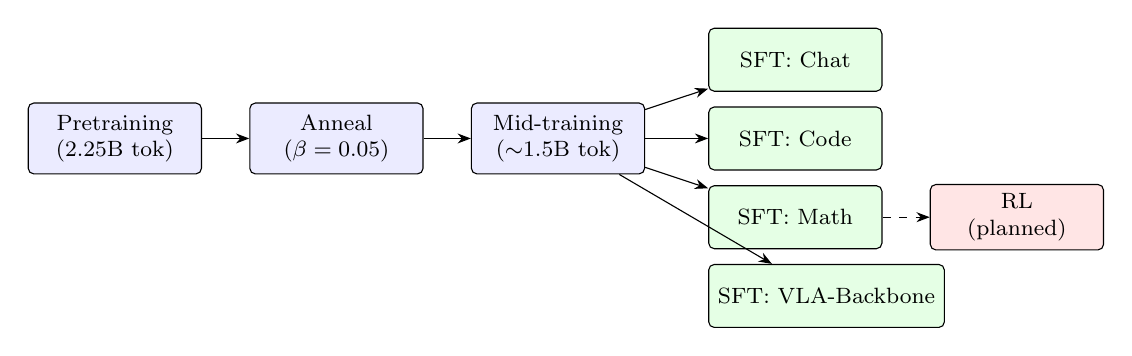
\begin{tikzpicture}[
  >=Stealth,
  block/.style={draw, rounded corners=2pt, minimum width=22mm, minimum height=9mm, fill=blue!8, align=center, font=\footnotesize},
  sft/.style={draw, rounded corners=2pt, minimum width=22mm, minimum height=8mm, fill=green!10, align=center, font=\footnotesize},
  rl/.style={draw, rounded corners=2pt, minimum width=22mm, minimum height=8mm, fill=red!10, align=center, font=\footnotesize},
]
\node[block] (s1) {Pretraining\\(2.25B tok)};
\node[block, right=6mm of s1] (s2) {Anneal\\($\beta = 0.05$)};
\node[block, right=6mm of s2] (s3) {Mid-training\\($\sim$1.5B tok)};
\node[sft, right=8mm of s3, yshift=10mm] (chat) {SFT: Chat};
\node[sft, right=8mm of s3] (code) {SFT: Code};
\node[sft, right=8mm of s3, yshift=-10mm] (math) {SFT: Math};
\node[sft, right=8mm of s3, yshift=-20mm] (vla) {SFT: VLA-Backbone};
\node[rl, right=6mm of math] (rl) {RL\\(planned)};
\draw[->] (s1) -- (s2);
\draw[->] (s2) -- (s3);
\draw[->] (s3) -- (chat);
\draw[->] (s3) -- (code);
\draw[->] (s3) -- (math);
\draw[->] (s3) -- (vla);
\draw[->, dashed] (math) -- (rl);
\end{tikzpicture}
\end{center}

Cross-stage transitions use the \texttt{--init-from} command-line flag, which
loads model weights but resets the optimizer state and step counter. This
ensures each new stage starts with a fresh learning-rate schedule, fresh
moments, and step-0 accounting (which matters for cosine schedules,
warmup, and benchmark snapshots). Same-stage resumption uses
\texttt{--resume}, which restores model, optimizer state, and step counter.

\subsection{Stage 1: Pretraining}
\label{sec:stage1}

\paragraph{Configuration.}
\texttt{config-ouro-stage1.yaml}.

\paragraph{Goal.}
Learn broad linguistic and factual representations from web-scale data at a
high learning rate, with the loop loss configured to keep per-step heads
useful ($\beta = 0.15$, \texttt{early\_exit\_threshold} disabled).

\paragraph{Optimization.}
AdamW~\cite{adamw} with $\beta_1 = 0.9$, $\beta_2 = 0.95$, $\epsilon = 10^{-8}$,
weight decay $0.1$ (decoupled from the LR) applied only to 2D parameters
(\texttt{ndim $\ge$ 2}); 1D parameters (RMSNorm scales, biases) use weight
decay 0. Gradient clipping at $\|g\|_2 \le 1.0$. Mixed-precision bf16
forward/backward, with optimizer state in fp32. Optional
\texttt{torch.compile} for kernel fusion.

\paragraph{Learning-rate schedule.}
A warmup--stable--cosine~\cite{wsd} schedule with peak LR
$\eta_{\max} = 3 \cdot 10^{-4}$ and minimum $\eta_{\min} = 3 \cdot 10^{-5}$,
warmup steps $W = 3000$, stable steps $S = 200{,}000$ (effectively never
reached at our max-step budget):
\begin{equation}
\eta(t) = \begin{cases}
\eta_{\max} \cdot t / W, & t < W \\[2pt]
\eta_{\max}, & W \le t < S \\[2pt]
\eta_{\min} + \tfrac{1}{2}(\eta_{\max} - \eta_{\min})\bigl(1 + \cos(\pi\, p(t))\bigr), & t \ge S
\end{cases}
\end{equation}
with $p(t) = (t - S) / (T_{\max} - S)$. With $T_{\max} = 75{,}000$ and
$S = 200{,}000$, the schedule remains in the ``stable'' regime for the
entirety of stage 1, leaving the decay to the explicit annealing stage.

\paragraph{Batch and token accounting.}
Per-GPU micro-batch of $16$ sequences of $2048$ tokens, with $G = 2$
gradient-accumulation steps and $W_s = 2$ data-parallel ranks, gives a
global batch of $16 \cdot 2 \cdot 2 = 64$ sequences and
$64 \cdot 2048 = 131{,}072$ tokens per optimizer step. The target of
$75{,}000$ steps corresponds to $\sim$9.8B tokens processed (multiple
epochs over the 2.25B-token corpus).

\paragraph{Hardware and throughput.}
Two NVIDIA RTX Pro 6000 (96 GB) over PCIe, NCCL backend for DDP.
Observed training throughput approximately $60{,}000$ tokens/second per GPU
in bf16 with \texttt{torch.compile}. Stage-1 wall-clock for 75k steps is
$\approx$54 hours.

\subsection{Stage 2: Continual-Training (CT) Annealing}

\paragraph{Configuration.}
\texttt{config-ouro-stage2-anneal.yaml}.

\paragraph{Goal.}
A continual-pretraining phase~\cite{ouro2025} that uses a substantially
lower learning rate and a relaxed KL coefficient. The intent is to
\emph{polish} the base model rather than introduce new knowledge.

\paragraph{Hyperparameters.}
LR cosine-annealed from $3 \cdot 10^{-5}$ to $3 \cdot 10^{-6}$ over 8{,}000
steps, warmup 200 steps, $\beta = 0.05$, and \texttt{early\_exit\_threshold
$= 0.85$} (used for inference/export; inline training benchmarks disable early
exit and evaluate full $R=4$ recurrence). The reduced $\beta$ permits the exit
distribution to specialize without forcing the per-step heads to remain fully
balanced, while the short horizon prevents over-training on the annealing mix.

\paragraph{Data.}
The annealing stage uses a dedicated high-quality corpus. The web component is
\texttt{HuggingFaceTB/dclm-edu} filtered to \texttt{edu\_int\_score >= 3},
chosen as an open high-quality Common Crawl replacement. It is combined with
\texttt{nvidia/Nemotron-CC-Math-v1} (\texttt{4plus}),
\texttt{LLM360/MegaMath} Web-Pro, \texttt{OpenCoder-LLM/opc-fineweb-code-corpus},
\texttt{OpenCoder-LLM/opc-fineweb-math-corpus}, and the OpenCoder annealing
corpus (algorithmic, synthetic snippet, and synthetic QA splits). This keeps
stage~2 as a genuine cleaner-data CT anneal while reserving instruction-heavy
Q/A and CoT data for stage~3.

\paragraph{Inline evaluation.}
Every 1000 optimizer steps we run the multiple-choice harness on a moderate
budget (200 examples per task, 20 validation perplexity batches) and log
the results to \texttt{runs/.../benchmarks/stepXXXXXXX.json} and to W\&B as
\texttt{bench/*}.

\subsection{Stage 3: Mid-Training}

\paragraph{Configuration.}
\texttt{config-ouro-stage3-midtrain.yaml}.

\paragraph{Goal.}
Mid-training~\cite{midtrain2025,springer-midtrain} bridges broad pretraining
and downstream SFT by training on a curated mixture of more targeted data
(code, math, Q/A, CoT) while replaying a fraction of the original
pretraining distribution to prevent forgetting.

\paragraph{Mixture (target $\sim$1.5B tokens).}
\begin{itemize}[noitemsep,leftmargin=*]
  \item 30\% code: CodeParrot-clean
  \item 25\% math: Open-Web-Math
  \item 25\% Q/A and CoT: MetaMathQA, OpenMathInstruct-2, OpenOrca, Alpaca-Cleaned
  \item 20\% replay: $\sim$300M tokens randomly sampled from
    \texttt{data/stage1-smollm/train.bin} via a new
    \texttt{replay\_bin} source type in \texttt{download\_data.py}
\end{itemize}

\paragraph{Hyperparameters.}
LR cosine $1 \cdot 10^{-5} \to 1 \cdot 10^{-6}$, warmup 300 steps, $\beta = 0.03$, 20{,}000 steps.

\subsection{Stage 4: Parallel Specialist SFT}

All four SFT branches are initialized from
\texttt{runs/rex-ouro-midtrain/ckpt\_final.pt} via \texttt{--init-from} and
trained independently. Each uses cosine-decayed LR
$2 \cdot 10^{-5} \to 2 \cdot 10^{-6}$, warmup 100 steps, weight decay $0.01$
(lower than pretraining to reduce drift), $\beta = 0.02$, and up to 8000
optimizer steps (10{,}000 for VLA).

\subsubsection{\textsc{Rex1-Chat}}

A general instruct SFT on OpenHermes-2.5, UltraChat-200k (SFT split),
SmolTalk, and Dolly-15k. All sources are formatted with the chat schema
\texttt{<|system|>}, \texttt{<|user|>}, \texttt{<|assistant|>}, supplied by
the \texttt{conversation\_column} mechanism in \texttt{download\_data.py}.

\subsubsection{\textsc{Rex1-Code}}

A code and tool-calling SFT mix: tool-calling (Glaive
\texttt{function-calling-v2}, Hermes function-calling, xLAM-60k), Python
instruction (Alpaca-formatted), Code-Feedback, Glaive code-assistant, and
Evol-Instruct-Code. Outputs may include \texttt{<tool\_call>\{...\}</tool\_call>}
spans followed by \texttt{<|tool|>} result blocks and a final
\texttt{<|assistant|>} response, providing a uniform multi-turn format.

\subsubsection{\textsc{Rex1-Math}}

A step-by-step math SFT: MetaMathQA, OpenMathInstruct-2, Orca-Math-Word-Problems,
NuminaMath-CoT. All formatted with explicit reasoning chains in the
\texttt{<|assistant|>} field, preparing the model for sparse verifiable-reward
RL in stage 5.

\subsubsection{\textsc{Rex1-VLA-Backbone}}

\paragraph{Motivation.}
A vision–language–action system requires a language backbone that already
understands imperative robot commands, spatial relations, and procedural
plans. Standard chat SFT trains the model toward conversational dialogue,
which is not the desired behavior when the LM serves as the policy
component of a robotic system.

\paragraph{Mixture (target $\sim$800M--1.2B tokens).}
\begin{itemize}[noitemsep,leftmargin=*]
  \item 35\% manipulation language with actions: ALFWorld trajectories
    (function-calling format) and ALFRED step/action pairs
  \item 25\% spatial reasoning: SpartQA queries joined with their ground-truth
    answers via a custom \texttt{spartqa\_joined} source type
  \item 20\% procedural plans: Cosmopedia WikiHow tutorials (long-form
    decomposition of physical tasks)
  \item 20\% replay from the mid-training bin
\end{itemize}

\paragraph{Scope.}
This stage is \emph{strictly text-only}. No images or visual encoders are
introduced. The branch outputs a checkpoint that downstream VLA work
(vision encoder + projector + action head) can build on.

\subsection{Stage 5: Reinforcement Learning (Planned)}

\paragraph{\textsc{Rex1-Math} (verifiable rewards).}
GRPO/RLOO~\cite{grpo} with $R = 1$ for correct final answer and $R = 0$
otherwise. Answer extraction uses a deterministic parser
(\texttt{boxed\{\}}, ``Answer: \dots'', or trailing numeric). Prompt pool drawn
from MetaMathQA / NuminaMath training splits; evaluation held out on GSM8K
test, MATH-500, and AIME problem sets.

\paragraph{\textsc{Rex1-Code} (unit-test rewards).}
Sandboxed unit-test execution, with reward $=$ fraction of passing tests.
Prompts drawn from HumanEval+ / MBPP+ style problem sets.

\paragraph{\textsc{Rex1-Chat} (preference optimization).}
DPO~\cite{dpo} on UltraFeedback-style preference pairs; reward-model-free.

These stages are designed and configured but not yet integrated into the
release training loop, and are not evaluated in this report.

%==============================================================================
\section{Data Engineering}
%==============================================================================

\subsection{Tokenization and Packing}

All training data is converted to packed \texttt{int32} token streams
(\texttt{train.bin}, \texttt{val.bin}). Each document is tokenized with the
SmolLM2-360M tokenizer, an EOS token is appended, and the resulting integer
sequence is written to the binary file. Documents are read by a
memory-mapped \texttt{numpy.memmap} array at training time; the data loader
slices contiguous windows of length \texttt{block\_size = 2048} with
\texttt{stride = 2048} (non-overlapping).

This format is simple, low-overhead, and avoids tokenization at training
time. Per-source token and document counts are written to a
\texttt{dataset\_meta.yaml} sidecar, enabling exact reproducibility of the
mix.

\subsection{Source Specification}

Sources are declared in YAML. Three primary modes are supported:

\paragraph{Flat text columns.}
The source provides a string column (e.g., \texttt{text}, \texttt{content})
that is tokenized directly.

\paragraph{Templates.}
A Python format string (\texttt{text\_template}) with placeholders
referencing source columns. Missing columns are filled with empty strings
via a custom \texttt{\_SafeFormatDict}. This is used to convert structured
data (Q/A pairs, ALFRED step records) into chat-formatted text.

\paragraph{Multi-turn conversations.}
A \texttt{conversation\_column} identifies a list of turn dictionaries with
\texttt{role}/\texttt{from} and \texttt{content}/\texttt{value} fields.
Role aliases (\texttt{human $\to$ user}, \texttt{gpt $\to$ assistant},
\texttt{function $\to$ tool}) normalize ShareGPT-style data to our chat
schema. The serialization uses \texttt{<|system|>}, \texttt{<|user|>},
\texttt{<|assistant|>}, \texttt{<|tool|>} delimiters and a default system
prompt from the YAML.

\subsection{Inter-Stage Replay}

A new source type, \texttt{replay\_bin}, samples \emph{token chunks}
directly from previous stages' packed bins without re-tokenizing. Given a
\texttt{replay\_bin} path and a \texttt{max\_train\_tokens} budget, the
downloader memory-maps the file, draws uniformly random
$[\texttt{chunk\_min}, \texttt{chunk\_max}]$-length contiguous slices, and
appends them to the new stage's training bin until the budget is met.

This makes anti-forgetting cheap: stage-3 mid-training and the
\textsc{Rex1-VLA-Backbone} branch both replay 20\% of their training token
budget from earlier-stage bins. Because chunks come from packed sequences,
the replay distribution matches the original training distribution exactly.

\subsection{SpartQA Custom Joiner}

The SpartQA spatial QA dataset on HuggingFace
(\texttt{mteb/SpartQA}) is published as three separate splits
(\texttt{queries}, \texttt{corpus}, \texttt{qrels}). A custom source type
\texttt{spartqa\_joined} loads all three, builds query- and document-ID
lookup tables, joins on the \texttt{qrels} relation, and emits chat-formatted
SFT examples. This pattern generalizes to other relevance-style datasets
that lack a direct text-answer column.

\subsection{Stage-1 Corpus Realized Composition}

The actual stage-1 token counts (from \texttt{dataset\_meta.yaml}) are
shown in Table~\ref{tab:stage1-data}.

\begin{table}[h]
  \centering
  \caption{Realized stage-1 corpus composition (SmolLM2 tokens).}
  \label{tab:stage1-data}
  \footnotesize
  \begin{tabular}{lrr}
    \toprule
    Source & Train docs & Train tokens \\
    \midrule
    FineWeb-Edu & 900{,}000 & 943.7M \\
    FineWeb (sample-10BT) & 350{,}000 & 249.8M \\
    Cosmopedia (7 configs: web, khanacademy, openstax, auto-math, stanford, wikihow) & 550{,}000 & $\sim$400M \\
    Wikipedia (en, 2023-11-01) & 150{,}000 & $\sim$140M \\
    Open-Web-Math & 120{,}000 & 265.3M \\
    CodeParrot-clean & 70{,}000 & 201.7M \\
    TinyStories & 300{,}000 & 67.3M \\
    WikiText-103 & 100{,}000 & 10.8M \\
    arXiv abstracts & 50{,}000 & 18.4M \\
    \midrule
    \textbf{Total} & \textbf{2{,}449{,}123} & \textbf{2{,}246.6M} \\
    \bottomrule
  \end{tabular}
\end{table}

%==============================================================================
\section{Training Infrastructure}
%==============================================================================

\subsection{Software Stack}

PyTorch~$\ge$2.2, HuggingFace \texttt{transformers} and \texttt{datasets},
\texttt{wandb} for logging, \texttt{lm-eval}~\cite{lm-eval-harness} as an
optional standardized evaluation harness, NumPy for memory-mapped token
arrays, \texttt{torch.compile} for kernel fusion.

\subsection{Distributed Training}

Multi-GPU training is launched with
\texttt{torchrun --standalone --nproc\_per\_node=2 train.py}. Setup:

\begin{itemize}[noitemsep,leftmargin=*]
  \item Each rank initializes its CUDA device based on \texttt{LOCAL\_RANK}.
  \item The tokenizer is loaded on rank 0 and broadcast to all ranks via
    \texttt{dist.broadcast\_object\_list}.
  \item Data is sharded by \texttt{DistributedSampler} with
    \texttt{drop\_last=True} so all ranks see identical batch counts per
    epoch.
  \item The model is wrapped with \texttt{DistributedDataParallel} after
    optimizer and (optional) compile.
  \item Evaluation (perplexity or the multi-choice benchmark suite) runs
    only on rank 0 with the DDP wrapper \emph{unwrapped} to a vanilla module.
    A subsequent \texttt{dist.barrier()} re-synchronizes ranks.
\end{itemize}

The unwrap step is necessary because the eval path runs many small forward
passes whose batch sizes differ from the training batch. Calling these
through DDP causes the NCCL all-reduce to deadlock when only rank~0 is
issuing them. By calling \texttt{unwrap\_model(model)} and running eval as a
local operation, we sidestep the deadlock cleanly while still using the
trained weights.

\subsection{Mixed-Precision and Compilation}

Forward and backward passes run in bfloat16 (no GradScaler since bf16 has
sufficient exponent range). Optimizer state remains in float32.
\texttt{torch.compile(model)} is applied after \texttt{init\_from} but before
the DDP wrap, providing $\sim$15--20\% throughput improvement on our GPUs.

\subsection{Checkpointing}

Training checkpoints are PyTorch \texttt{.pt} files containing:
\begin{itemize}[noitemsep,leftmargin=*]
  \item \texttt{model}: state dict (no DDP wrapper)
  \item \texttt{optimizer}: AdamW state
  \item \texttt{step}: integer step counter
  \item \texttt{model\_config}: \texttt{RexConfig.to\_dict()}
  \item \texttt{config}: full YAML stage config
\end{itemize}
This is sufficient to rebuild the model and (optionally) the optimizer at
any stage. Two CLI modes load checkpoints:

\begin{description}[leftmargin=*]
\item[\texttt{--resume PATH}] Restore model weights, optimizer state, and
step counter. Use within a single stage to recover from interruption.
\item[\texttt{--init-from PATH}] Restore model weights only; optimizer is
freshly initialized and step counter starts at 0. Use across stage
boundaries to apply the new stage's LR schedule cleanly.
\end{description}

Saved checkpoints follow the convention
\texttt{runs/<stage>/ckpt\_stepXXXXX.pt} every \texttt{save\_every} steps
and \texttt{ckpt\_final.pt} at the end of the run.

\subsection{Export}

\texttt{export\_hf.py} converts a training checkpoint into a HuggingFace-style
folder (\texttt{config.json}, \texttt{pytorch\_model.bin}, model card) so
that the model can be loaded with \texttt{RexForCausalLM.from\_pretrained}
or shared via the HuggingFace Hub.

\subsection{Observability}

Each training run logs to Weights \& Biases (when enabled):
\texttt{train/loss}, \texttt{train/task\_loss}, per-step losses
\texttt{train/step\{r\}\_loss}, \texttt{train/kl\_uniform},
\texttt{train/exit\_prob\_step\{r\}}, \texttt{train/lr},
\texttt{train/tokens\_per\_second}, \texttt{train/tokens\_seen}. Inline
benchmark results are logged under the \texttt{bench/*} namespace and
mirrored to JSON snapshots on disk.

%==============================================================================
\section{Evaluation Protocol}
%==============================================================================

\subsection{Validation Perplexity}

Standard token-averaged cross-entropy on a held-out packed \texttt{val.bin}.
With batch size 2 and \texttt{val\_batches} iterations, the metric is
\begin{equation}
\mathrm{PPL}_{\mathrm{val}} = \exp\left(\frac{1}{N_{\mathrm{val}}}\sum_{i=1}^{N_{\mathrm{val}}} \mathcal{L}_i\right),
\end{equation}
where $\mathcal{L}_i$ is the model's final-step cross-entropy on the $i$-th
validation batch. Because the validation bin is sampled from the same
distribution as the training bin for each stage, this metric tracks training
progress more reliably than zero-shot benchmarks but is not directly
comparable across stages with different data.

\subsection{Continuation-Loss Multiple-Choice Scoring}

Standard multiple-choice benchmarks (HellaSwag, ARC-E/C, SciQ, OpenBookQA,
WinoGrande, PIQA, BoolQ) are evaluated via a continuation-loss
ranking~\cite{eval-harness}: for each candidate continuation $c_i$ to a
prompt $p$, we compute the average per-token cross-entropy
$\mathcal{L}(c_i \mid p)$ on the continuation tokens only (prompt tokens are
masked with \texttt{ignore\_index = -100}), and predict
$\hat{c} = \arg\min_i \mathcal{L}(c_i \mid p)$.

This is functionally similar to \texttt{lm-eval-harness}'s
\texttt{loglikelihood} task in length-normalized mode (\texttt{acc\_norm}),
but our implementation:
\begin{itemize}[noitemsep,leftmargin=*]
  \item normalizes by the number of continuation tokens (not the byte length
    or the character length)
  \item uses the model's training-time recurrence depth ($R = 4$) without
    early exit
  \item applies no answer-letter parsing or special prompt formatting
    beyond a minimal ``Question: \ldots Answer:'' template for ARC/SciQ.
\end{itemize}
Absolute numbers are therefore not directly comparable to published Pythia
or SmolLM2 tables, which use \texttt{lm-eval-harness} settings. We report
both raw and length-normalized harness values for the comparison models
where available, and we are clear about the methodological gap.

\subsection{Tasks Implemented}

\begin{table}[h]
  \centering
  \caption{Evaluation tasks supported by \texttt{benchmark.py}.}
  \label{tab:tasks}
  \footnotesize
  \begin{tabular}{lll}
    \toprule
    Task & HF dataset & Metric \\
    \midrule
    HellaSwag & \texttt{Rowan/hellaswag} & 4-way MC continuation loss \\
    ARC-Easy & \texttt{ai2\_arc/ARC-Easy} & MC continuation loss \\
    ARC-Challenge & \texttt{ai2\_arc/ARC-Challenge} & MC continuation loss \\
    SciQ & \texttt{allenai/sciq} & 4-way MC continuation loss \\
    OpenBookQA & \texttt{openbookqa/main} & MC continuation loss \\
    WinoGrande & \texttt{winogrande/winogrande\_xl} & 2-way MC continuation loss \\
    PIQA & \texttt{piqa} & 2-way MC continuation loss \\
    BoolQ & \texttt{google/boolq} & MC over \{yes, no\} \\
    val\_ppl & packed validation bin & perplexity \\
    \bottomrule
  \end{tabular}
\end{table}

%==============================================================================
\section{Preliminary Results}
%==============================================================================

\subsection{Stage 1 @ Step 40{,}000}

The reported checkpoint \texttt{runs/rex-ouro-stage1/ckpt\_step40000.pt}
corresponds to approximately $40{,}000 \cdot 131{,}072 \approx 5.24\mathrm{B}$
tokens processed (multiple epochs over the 2.25B-token stage-1 corpus).
Benchmark numbers are reported on 200 examples per task and 20 validation
batches (Table~\ref{tab:stage1-40k}).

\begin{table}[h]
  \centering
  \caption{\REX stage-1 @ 40k steps under continuation-loss MC scoring
  (200 examples per task), compared to Pythia-410M
  (\texttt{lm-eval-harness} \texttt{acc\_norm} where available).}
  \label{tab:stage1-40k}
  \begin{tabular}{lcc}
    \toprule
    Task & \REX @ 40k (ours) & Pythia-410M (lm-eval, fully trained) \\
    \midrule
    HellaSwag & 35.5\% & 33.7\% (acc) / 40.6\% (acc\_norm) \\
    ARC-Easy & 43.5\% & $\sim$48--49\% \\
    SciQ & 55.0\% & $\sim$89\% (lm-eval; not directly comparable, see text) \\
    OpenBookQA & 23.5\% & 18.0\% (acc) / 29.4\% (acc\_norm) \\
    Val PPL & 20.9 & --- \\
    \bottomrule
  \end{tabular}
\end{table}

A few observations:

\begin{itemize}[leftmargin=*]
  \item Despite $\sim$58$\times$ fewer pretraining tokens and $\sim$35\%
    fewer parameters than fully-trained Pythia-410M, \REX is already
    \textbf{competitive on HellaSwag and ARC-Easy} at the 40k checkpoint.
  \item SciQ shows the largest gap. We believe this is partly a
    methodological artifact: SciQ is sensitive to the exact prompt template
    and length-normalization used. Our raw continuation-loss
    score (55.0\%) on SciQ corresponds to a much higher accuracy under
    standard lm-eval scoring; calibrating this is left to a future revision.
  \item OpenBookQA is within $\sim$6 points of Pythia's \texttt{acc\_norm},
    which is a strong relative position given the data budget gap.
\end{itemize}

\subsection{Stage 2 Anneal: Active High-Quality Run}

The active stage-2 run initializes from
\texttt{runs/rex-ouro-stage1/ckpt\_step40000.pt} and trains for 8{,}000
optimizer steps on a dedicated high-quality annealing corpus. The run uses
full $R=4$ recurrence for inline benchmarks while retaining
\texttt{early\_exit\_threshold = 0.85} in the model configuration for inference.

\begin{table}[h]
  \centering
  \caption{Current stage-2 annealing data mixture.}
  \label{tab:stage2-data}
  \footnotesize
  \begin{tabular}{llc}
    \toprule
    Component & Dataset / filter & Target share \\
    \midrule
    HQ web & \texttt{HuggingFaceTB/dclm-edu}, \texttt{edu\_int\_score >= 3} & 40\% \\
    HQ math & \texttt{nvidia/Nemotron-CC-Math-v1}, \texttt{4plus} & 20\% \\
    HQ math web & \texttt{LLM360/MegaMath} Web-Pro & 15\% \\
    HQ code & \texttt{OpenCoder-LLM/opc-fineweb-code-corpus} & 12\% \\
    HQ math recall & \texttt{OpenCoder-LLM/opc-fineweb-math-corpus} & 8\% \\
    Code anneal & OpenCoder algorithmic / snippet / QA annealing splits & 5\% \\
    \bottomrule
  \end{tabular}
\end{table}

Inline benchmarks are logged every 1{,}000 optimizer steps with 200 examples per
multiple-choice task and 20 validation-perplexity batches. Checkpoints are saved
every 2{,}000 steps so the final stage-3 initialization can be selected from the
best stage-2 benchmark point rather than blindly taking the last checkpoint.

%==============================================================================
\section{Inference and Deployment}
%==============================================================================

\subsection{Generation}

\REX implements standard autoregressive generation with optional KV caching
(\texttt{use\_kv\_cache=True}). Sampling controls include temperature, top-$k$,
and no-repeat-$n$-gram. The KV cache is structured per-recurrence-step (a
list of length $R$), allowing early exit during prefill if
\texttt{early\_exit\_threshold} is set.

When \texttt{local\_block\_size > 0}, KV caching is disabled because the
block-local mask breaks the standard cache assumption that past keys/values
are reused across decoding steps; this is documented as a caveat.

\subsection{Early Exit at Inference}

At inference, after step $r$ the model checks the cumulative survival mass
and breaks out of the recurrence loop if it exceeds $\tau$ (default
$\tau = 0.85$). This reduces effective FLOPs per token. Because the gate
output is a learned function of the latent state, the effective compute
adapts per-input: simple continuations exit early; harder predictions use
more depth.

We expect early exit to deliver meaningful latency wins on phone-class
inference engines, but a full latency study (with quantization) is left to
follow-up work.

\subsection{Quantization}

\REX exports cleanly to standard quantization formats:

\begin{itemize}[noitemsep,leftmargin=*]
  \item GGUF: convert via \texttt{llama.cpp}-style flows after exporting to
    a HuggingFace-compatible folder. Recommended Q4\_K\_M for general use,
    Q5\_K\_M for higher fidelity.
  \item AWQ~\cite{awq}: standard activation-aware weight quantization should
    apply with no architecture-specific modifications.
\end{itemize}

We do not report post-quantization benchmark numbers in this release.

%==============================================================================
\section{Model Family Summary}
%==============================================================================

\begin{table}[h]
  \centering
  \caption{Planned \REX release artifacts.}
  \label{tab:family}
  \footnotesize
  \begin{tabular}{lllp{5.5cm}}
    \toprule
    Artifact & Source stage & Status & Use case \\
    \midrule
    \REX-Base & End of stage 2 & Pending stage 2 completion & Completion, further pretraining, research base \\
    \REX-Chat & Stage 4 chat SFT & Config ready & On-device general assistant \\
    \REX-Code & Stage 4 code SFT & Config ready & Coding + tool calling \\
    \REX-Math & Stage 4 math SFT & Config ready; RL follow-up planned & Math reasoning \\
    \REX-VLA-Backbone & Stage 4 VLA SFT & Config ready & Robotics LM core for VLA \\
    \bottomrule
  \end{tabular}
\end{table}

%==============================================================================
\section{Reproducibility}
%==============================================================================

The full pipeline reproduces with the following commands.

\begin{lstlisting}[language=bash]
# Build stage-1 packed bins (~hours, depending on bandwidth)
python download_data.py --config config-ouro-stage1.yaml

# Stage 1: pretraining
torchrun --standalone --nproc_per_node=2 train.py \
    --config config-ouro-stage1.yaml

# Stage 2: build HQ annealing bins and CT anneal from a stage-1 checkpoint
python download_data.py --config config-ouro-stage2-anneal.yaml
torchrun --standalone --nproc_per_node=2 train.py \
    --config config-ouro-stage2-anneal.yaml \
    --init-from runs/rex-ouro-stage1/ckpt_step40000.pt

# Stage 3: mid-training
python download_data.py --config config-ouro-stage3-midtrain.yaml
torchrun --standalone --nproc_per_node=2 train.py \
    --config config-ouro-stage3-midtrain.yaml \
    --init-from runs/rex-ouro-stage2/ckpt_final.pt

# Stage 4: parallel specialist SFT
python download_data.py --config config-ouro-stage4-chat.yaml
torchrun --standalone --nproc_per_node=2 train.py \
    --config config-ouro-stage4-chat.yaml \
    --init-from runs/rex-ouro-midtrain/ckpt_final.pt

# Standalone benchmark
python benchmark.py \
    --config config-ouro-stage1.yaml \
    --checkpoint runs/rex-ouro-stage1/ckpt_step40000.pt \
    --tasks hellaswag,arc_easy,sciq,openbookqa,val_ppl \
    --mc-examples 200 --val-batches 20

# HuggingFace export
python export_hf.py --checkpoint runs/rex1-chat/ckpt_final.pt \
    --config config-ouro-stage4-chat.yaml \
    --out-dir exports/rex1-chat --model-name REX1-Chat
\end{lstlisting}

All YAML configurations referenced above (\texttt{config-ouro-stage1.yaml},
\ldots, \texttt{config-ouro-stage4-vla-backbone.yaml}) are included in the
release repository alongside \texttt{train.py}, \texttt{model.py},
\texttt{benchmark.py}, \texttt{download\_data.py}, \texttt{export\_hf.py},
\texttt{inference.py}, and \texttt{eval\_lm\_harness.py}.

%==============================================================================
\section{Limitations}
%==============================================================================

\paragraph{Scale.} \REX is a $\sim$300M-parameter model trained on a few
billion tokens. It is not competitive with current frontier models on most
generative tasks. Performance numbers in this report should be read as
indicators of pipeline correctness and the relative cost of looped vs.\
non-looped designs at this scale, not as a state-of-the-art claim.

\paragraph{Context length.} All stages use $T = 2048$. We expect context to
extend cleanly to 4096--8192 via RoPE base scaling and a brief long-context
fine-tuning pass, but this is future work.

\paragraph{Evaluation methodology.} Our continuation-loss MC scoring differs
from standard \texttt{lm-eval-harness} settings. Numbers in this report
should not be directly compared to published Pythia/SmolLM2 tables without
care. A re-evaluation under harness defaults is planned.

\paragraph{Annealing data.} Stage~2 uses a curated high-quality annealing mix:
DCLM-Edu with \texttt{edu\_int\_score >= 3}, Nemotron-CC-Math \texttt{4plus},
MegaMath-Web-Pro, and OpenCoder code/math/annealing data. Because this changes
the validation distribution, stage-2 validation perplexity should be
interpreted as a within-run signal rather than directly compared to stage~1
validation perplexity.

\paragraph{RL and vision.} Stages 5 (RL) and any vision-language-action
training are designed and discussed but not implemented in this release.
\REX-VLA-Backbone is a text-only steering pass; full VLA training is left to
downstream collaborators.

\paragraph{Bias and safety.} No systematic safety evaluation has been
performed. As with any LM trained on web data, \REX may produce harmful,
biased, or factually incorrect outputs. Users are expected to apply
appropriate filters and review for downstream deployments.

%==============================================================================
\section{Future Work}
%==============================================================================

\begin{enumerate}[leftmargin=*]
  \item \textbf{Finish stage 1 to 75k steps} and produce a fully-annealed
    \REX-Base checkpoint for release.
  \item \textbf{Long-context fine-tune} to 4096 and 8192 tokens via RoPE
    base scaling + brief continued pretraining on long documents.
  \item \textbf{Integrate stage 5 RL} using TRL for DPO and a custom GRPO
    trainer for verifiable-reward math and code rollouts.
  \item \textbf{VLM/VLA stack} on top of \REX-VLA-Backbone: small vision
    encoder (MobileCLIP / SigLIP-400M), MLP projector, optional action head,
    with $\le$200M visual-instruction tokens.
  \item \textbf{Ablations} of recurrence depth $R$, $\beta$ schedule, sandwich
    norm, and exit-gate parameterization, to characterize the LoopLM design
    space at small scale.
  \item \textbf{Quantized inference benchmarks} (Q4\_K\_M, AWQ) on
    representative edge devices, including latency vs.\
    \texttt{early\_exit\_threshold} curves.
  \item \textbf{Harness re-evaluation.} Re-run all benchmarks via
    \texttt{lm-eval-harness} for direct comparison to public model tables.
\end{enumerate}

%==============================================================================
\section{Conclusion}
%==============================================================================

\REX is a small, fully open, parameter-efficient recurrent looped language
model trained through a five-stage pipeline---pretraining, CT annealing,
mid-training, parallel specialist SFT, and (planned) RL. At a research-scale
compute budget on two consumer GPUs, the model already shows competitive
multiple-choice reasoning numbers at the 40k pretraining checkpoint, and the
active cleaner-data CT anneal turns that checkpoint into the base for
mid-training. We release the full training stack,
all stage configurations, the data engineering tools, and this technical
report so that the model can be reproduced, modified, and used as a base
for downstream specialization---particularly the text-only
\REX-VLA-Backbone branch, which is designed to serve as the language core
of future vision-language-action systems on edge hardware.

%==============================================================================
\section*{Acknowledgments}
%==============================================================================

We build directly on the Ouro looped-LM framework and the SmolLM2 tokenizer.
We rely on open data and code from the FineWeb, Cosmopedia, Open-Web-Math,
CodeParrot, TinyStories, Wikipedia, arXiv, OpenHermes, UltraChat, Glaive,
Hermes, xLAM, MetaMathQA, OpenMathInstruct, Orca-Math, NuminaMath,
Code-Feedback, ALFRED, ALFWorld, SpartQA, and many other community
projects. We thank the broader open-source ML community for the
infrastructure (PyTorch, HuggingFace, W\&B) that makes work at this scale
possible.

%==============================================================================
\begin{thebibliography}{99}
\bibitem{ouro2025}
ByteDance Research.
\newblock Scaling Latent Reasoning via Looped Language Models (Ouro).
\newblock \url{https://arxiv.org/abs/2510.25741}, 2025.

\bibitem{deth}
J.~Geiping et al.
\newblock Scaling up Test-Time Compute with Latent Reasoning: A Recurrent Depth Approach.
\newblock arXiv, 2024.

\bibitem{universal-transformer}
M.~Dehghani et al.
\newblock Universal Transformers.
\newblock ICLR, 2019.

\bibitem{albert}
Z.~Lan et al.
\newblock ALBERT: A Lite BERT for Self-Supervised Learning of Language Representations.
\newblock ICLR, 2020.

\bibitem{block-recurrent-transformer}
D.~Hutchins et al.
\newblock Block-Recurrent Transformers.
\newblock NeurIPS, 2022.

\bibitem{coconut}
S.~Hao et al.
\newblock Training Large Language Models to Reason in a Continuous Latent Space (Coconut).
\newblock arXiv, 2024.

\bibitem{quietstar}
E.~Zelikman et al.
\newblock Quiet-STaR: Language Models Can Teach Themselves to Think Before Speaking.
\newblock arXiv, 2024.

\bibitem{midtrain2025}
S.~Wang et al.
\newblock Mid-Training of Large Language Models: A Survey.
\newblock \url{https://arxiv.org/abs/2510.06826}, 2025.

\bibitem{midtrain-survey-23081}
Various.
\newblock A Survey on LLM Mid-Training.
\newblock \url{https://arxiv.org/abs/2510.23081}, 2025.

\bibitem{springer-midtrain}
Springer et al.
\newblock Midtraining Bridges Pretraining and Posttraining Distributions.
\newblock \url{https://arxiv.org/abs/2510.14865}, 2025.

\bibitem{olmo2}
AI2 OLMo Team.
\newblock OLMo 2: A Truly Open Language Model.
\newblock AI2, 2024.

\bibitem{nemotron}
NVIDIA.
\newblock Nemotron-4 / Nemotron Pretraining Data Report.
\newblock NVIDIA, 2024.

\bibitem{llama3}
Meta.
\newblock The Llama 3 Herd of Models.
\newblock Meta AI, 2024.

\bibitem{yi}
01.AI.
\newblock Yi: Open Foundation Models by 01.AI.
\newblock 01.AI, 2024.

\bibitem{codellama}
Rozi\`ere et al.
\newblock Code Llama: Open Foundation Models for Code.
\newblock Meta AI, 2023.

\bibitem{smollm2}
HuggingFace TB.
\newblock SmolLM2: When Smol Goes Big.
\newblock \url{https://huggingface.co/HuggingFaceTB/SmolLM2-360M}, 2024.

\bibitem{pythia}
S.~Biderman et al.
\newblock Pythia: A Suite for Analyzing Large Language Models Across Training and Scaling.
\newblock ICML, 2023.

\bibitem{gqa}
J.~Ainslie et al.
\newblock GQA: Training Generalized Multi-Query Transformer Models from Multi-Head Checkpoints.
\newblock EMNLP, 2023.

\bibitem{rope}
J.~Su et al.
\newblock RoFormer: Enhanced Transformer with Rotary Position Embedding.
\newblock Neurocomputing, 2024.

\bibitem{rmsnorm}
B.~Zhang and R.~Sennrich.
\newblock Root Mean Square Layer Normalization.
\newblock NeurIPS, 2019.

\bibitem{swiglu}
N.~Shazeer.
\newblock GLU Variants Improve Transformer.
\newblock arXiv, 2020.

\bibitem{sandwich-norm}
T.~Liu et al.
\newblock Sandwich Layer Normalization (in Megatron-LM).
\newblock NVIDIA, 2021.

\bibitem{adamw}
I.~Loshchilov and F.~Hutter.
\newblock Decoupled Weight Decay Regularization.
\newblock ICLR, 2019.

\bibitem{wsd}
S.~Hu et al.
\newblock MiniCPM: Unveiling the Potential of Small Language Models with Scalable Training Strategies.
\newblock arXiv, 2024 (warmup--stable--decay schedule).

\bibitem{lm-eval-harness}
L.~Gao et al.
\newblock A Framework for Few-Shot Language Model Evaluation (\texttt{lm-eval-harness}).
\newblock EleutherAI, 2024.

\bibitem{eval-harness}
S.~Biderman et al.
\newblock Lessons From the Trenches on Reproducible Evaluation of Language Models.
\newblock arXiv, 2024.

\bibitem{rt2}
A.~Brohan et al.
\newblock RT-2: Vision-Language-Action Models Transfer Web Knowledge to Robotic Control.
\newblock CoRL, 2023.

\bibitem{openvla}
M.~Kim et al.
\newblock OpenVLA: An Open-Source Vision-Language-Action Model.
\newblock \url{https://openvla.github.io/}, 2024.

\bibitem{rt1}
A.~Brohan et al.
\newblock RT-1: Robotics Transformer for Real-World Control at Scale.
\newblock RSS, 2022.

\bibitem{octo}
Octo Model Team.
\newblock Octo: An Open-Source Generalist Robot Policy.
\newblock RSS, 2024.

\bibitem{alfred}
M.~Shridhar et al.
\newblock ALFRED: A Benchmark for Interpreting Grounded Instructions for Everyday Tasks.
\newblock CVPR, 2020.

\bibitem{alfworld}
M.~Shridhar et al.
\newblock ALFWorld: Aligning Text and Embodied Environments for Interactive Learning.
\newblock ICLR, 2021.

\bibitem{spartqa}
R.~Mirzaee et al.
\newblock SPARTQA: A Textual Question Answering Benchmark for Spatial Reasoning.
\newblock NAACL, 2021.

\bibitem{grpo}
Z.~Shao et al.
\newblock DeepSeekMath: Pushing the Limits of Mathematical Reasoning in Open Language Models (GRPO).
\newblock arXiv, 2024.

\bibitem{dpo}
R.~Rafailov et al.
\newblock Direct Preference Optimization: Your Language Model is Secretly a Reward Model.
\newblock NeurIPS, 2023.

\bibitem{awq}
J.~Lin et al.
\newblock AWQ: Activation-aware Weight Quantization for LLM Compression and Acceleration.
\newblock MLSys, 2024.

\end{thebibliography}

\appendix

%==============================================================================
\section{Full Hyperparameter Tables}
%==============================================================================

\subsection{Architecture}

\begin{table}[h]
  \centering
  \footnotesize
  \begin{tabular}{ll}
    \toprule
    Hyperparameter & Value \\
    \midrule
    Vocabulary size $V$ & 49{,}152 \\
    Context length $T$ & 2{,}048 \\
    Model dimension $d$ & 1{,}536 \\
    Number of blocks $N_l$ & 8 \\
    Recurrence steps $R$ & 4 \\
    Effective depth $R N_l$ & 32 \\
    Query heads $H$ & 16 \\
    KV heads $H_k$ & 4 \\
    Head dimension $d_h$ & 96 \\
    FFN dimension $d_{\mathrm{ffn}}$ & 3{,}968 \\
    Activation & SwiGLU \\
    Normalization & RMSNorm + sandwich \\
    Positional encoding & RoPE, $\theta = 50{,}000$ \\
    Embedding tying & yes \\
    Dropout & 0.0 \\
    Step embeddings & enabled \\
    Exit gate & enabled \\
    Early-exit threshold (inference, stage 2+) & 0.85 \\
    Total parameters & 269.0M \\
    \bottomrule
  \end{tabular}
\end{table}

\subsection{Stage Hyperparameters}

\begin{table}[h]
  \centering
  \footnotesize
  \begin{tabular}{lccccc}
    \toprule
    & Stage 1 & Stage 2 & Stage 3 & Stage 4 (each) & Stage 4 (VLA) \\
    & Pretrain & Anneal & Midtrain & SFT chat/code/math & VLA SFT \\
    \midrule
    Max steps & 75k & 8k & 20k & 8k & 10k \\
    Peak LR & 3e-4 & 3e-5 & 1e-5 & 2e-5 & 2e-5 \\
    Min LR & 3e-5 & 3e-6 & 1e-6 & 2e-6 & 2e-6 \\
    Warmup steps & 3000 & 200 & 300 & 100 & 100 \\
    LR schedule & WSD-cosine & cosine & cosine & cosine & cosine \\
    Stable steps & 200k & --- & --- & --- & --- \\
    Weight decay & 0.1 & 0.1 & 0.1 & 0.01 & 0.01 \\
    $\beta_1, \beta_2$ & 0.9, 0.95 & 0.9, 0.95 & 0.9, 0.95 & 0.9, 0.95 & 0.9, 0.95 \\
    Grad clip & 1.0 & 1.0 & 1.0 & 1.0 & 1.0 \\
    Exit-gate $\beta$ & 0.15 & 0.05 & 0.03 & 0.02 & 0.02 \\
    Early exit threshold & --- & 0.85 & 0.85 & 0.85 & 0.85 \\
    Micro batch & 16 & 16 & 16 & 16 & 16 \\
    Grad accum & 2 & 2 & 2 & 2 & 2 \\
    Global batch (seqs) & 64 & 64 & 64 & 64 & 64 \\
    Tokens/step & 131{,}072 & 131{,}072 & 131{,}072 & 131{,}072 & 131{,}072 \\
    Eval mode & val PPL & benchmarks & benchmarks & benchmarks & benchmarks \\
    Eval every & 2000 & 1000 & 2000 & 1000 & 1000 \\
    Save every & 5000 & 2000 & 5000 & 1000 & 1000 \\
    \bottomrule
  \end{tabular}
\end{table}

%==============================================================================
\section{Parameter Count Breakdown}
\label{app:params}
%==============================================================================

For the default \REX configuration (one set of 8 shared blocks; embeddings
tied):

\begin{table}[h]
  \centering
  \footnotesize
  \begin{tabular}{lr}
    \toprule
    Component & Parameters \\
    \midrule
    Token embedding $V \cdot d$ (tied with LM head) & 75{,}497{,}472 \\
    Per block: \\
    \quad pre-attn RMSNorm + post-attn RMSNorm & $2d = 3{,}072$ \\
    \quad QKV projections $(H + 2 H_k) d_h \cdot d$ & $(16 + 8) \cdot 96 \cdot 1536 = 3{,}538{,}944$ \\
    \quad attention output $d \cdot d$ & $2{,}359{,}296$ \\
    \quad pre-FFN RMSNorm + post-FFN RMSNorm & $2d = 3{,}072$ \\
    \quad SwiGLU $3 \cdot d \cdot d_{\mathrm{ffn}}$ & $3 \cdot 1536 \cdot 3968 = 18{,}284{,}544$ \\
    \quad block total & $24{,}188{,}928$ \\
    All $N_l = 8$ blocks & $193{,}511{,}424$ \\
    Final RMSNorm & $1{,}536$ \\
    Step embeddings $R \cdot d$ & $6{,}144$ \\
    Exit gate ($d + 1$) & $1{,}537$ \\
    \midrule
    \textbf{Total} & \textbf{$\approx$ 269.0M} \\
    \bottomrule
  \end{tabular}
\end{table}

%==============================================================================
\section{Example Data Formats}
%==============================================================================

\paragraph{Stage-1 web text.}
Documents are concatenated with an EOS token separator and packed into 2048-token windows.

\paragraph{Chat (\REX-Chat).}
\begin{lstlisting}
<|system|>
You are REX, a helpful and honest assistant. Answer clearly and concisely.
<|user|>
Explain RMSNorm in one paragraph.
<|assistant|>
RMSNorm normalizes activations by their root-mean-square...
\end{lstlisting}

\paragraph{Tool-calling (\REX-Code).}
\begin{lstlisting}
<|system|>
You are REX, an expert coding assistant with access to tools...
<|user|>
What's the current weather in Berlin?
<|assistant|>
<tool_call>{"name": "get_weather", "arguments": {"city": "Berlin"}}</tool_call>
<|tool|>
{"temperature_c": 12, "condition": "cloudy"}
<|assistant|>
It's currently 12 C and cloudy in Berlin.
\end{lstlisting}

\paragraph{ALFRED (\REX-VLA-Backbone).}
\begin{lstlisting}
<|system|>
You are a household robot controller in a simulated home.
<|user|>
Task: Cut an apple, cook a piece of the apple in a microwave, put the apple slice on the brown shelf.
Task type: pick_heat_then_place_in_recep
Step: 0
<|assistant|>
Action: LookDown
\end{lstlisting}

\paragraph{SpartQA (\REX-VLA-Backbone).}
\begin{lstlisting}
<|system|>
You are the language backbone for an embodied robot...
<|user|>
We have three blocks. Lets call them A, B and C. Block B is below A. Block A is below C...
What is below the black thing? a medium yellow square that is in block A or a medium yellow
square that is in block B?
<|assistant|>
both of them
\end{lstlisting}

\end{document}
